\section*{Problem 3}
\addcontentsline{toc}{section}{Problem 3}

\textbf{Statement:}

The point is selected in random at unit sphere $S^2 \subset \mathbb{R}^3$ and
then projected to the diameter. Find the probability that the distance from
the origin is more than $\frac{1}{2}$.

\noindent\textbf{Solution:}

We assume that the point is selected uniformly at the unit sphere, and that the
diameter is the $x$ axis.

Note that to project a point to the diameter we can just take the $x$ coordinate
of the point.

So the points with $x$ coordinate less than $-\frac{1}{2}$ or greater than
$\frac{1}{2}$ are the points that are more than $\frac{1}{2}$ away from the origin.

So similar to problem 2, we can solve this problem by finding the area of
the unit sphere made by the points with $x$ coordinate less than $-\frac{1}{2}$
or greater than $\frac{1}{2}$ and divide it by the area of the unit sphere.

We can notice that we just need to calculate the area of the unit sphere made
by the points with $x$ coordinate greater than $\frac{1}{2}$ and multiply it by
two to get the total area of the unit sphere made by the points with $x$ coordinate
less than $-\frac{1}{2}$ or greater than $\frac{1}{2}$.

To calculate this area just use the Spherical cap formula:

\begin{equation*}
    A = 2\pi R h
\end{equation*}

Where $R$ is the radius of the sphere and $h$ is the height of the cap.

In this case $R = 1$ and $h = 1 - \frac{1}{2} = \frac{1}{2}$.

\begin{figure}[H]
    \centering
    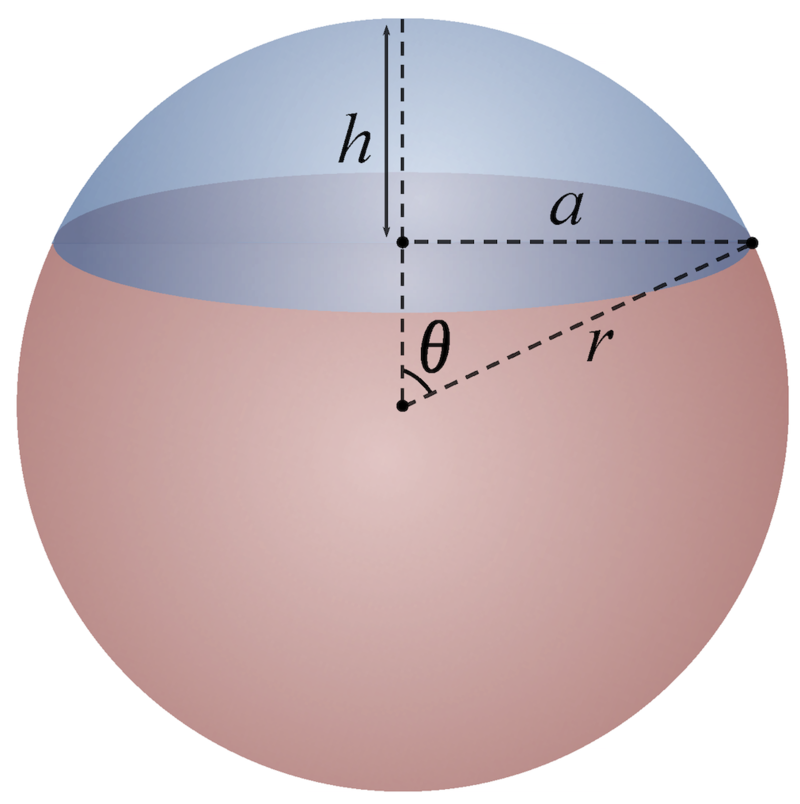
\includegraphics[width=0.5\textwidth]{images/spherical-cap.png}
\end{figure}

So the area of the unit sphere made by the points with $x$ coordinate greater
than $\frac{1}{2}$ is $2\pi \cdot 1 \cdot \frac{1}{2} = \pi$.

So the total area of the unit sphere made by the points with $x$ coordinate
less than $-\frac{1}{2}$ or greater than $\frac{1}{2}$ is $2\pi$.

Then the total area of the unit sphere is $4\pi$, by formula of the area of a
sphere ($4\pi R^2$).

So the probability is:

\begin{equation*}
    P( \text{distance from origin} > \frac{1}{2} ) = \frac{2\pi}{4\pi} = \frac{1}{2}
\end{equation*}